{\descr{Обчислити площу плоскої фігури, обмеженох данними лініями}}

$$
  \rho=2\sqrt{3}\cos\varphi,{\qquad} \rho=2\sin\varphi
$$

Якщо функція на відрізку  $[a; b]$  задана в параметричній формі
$x=x(t), y=y(t) , t \in [\varphi_1;\varphi_2]$ , де $x\varphi_1)=a, x=(\varphi_2)=b$ і функції $x(\varphi), y(\varphi)$
неперервно диференційовні на  $[t_1;t_2]$, то площа криволінійної трапеції дорівнює
$$S=\int^{\varphi_2}_{\varphi_1} y(\varphi)x'(\varphi) \d{\varphi}$$

Для визначеності, припустимо що параметричні рівняння $\begin{cases} \rho=2\sqrt{3}\cos\varphi \\ \rho=2\sin\varphi \end{cases}$ задають канонічний еліпс з центром на початку координат великою напівосью в точкі $2\sqrt{3}$ і короткою в точкі $2$.

\begin{figure}[h!]
  \centering
  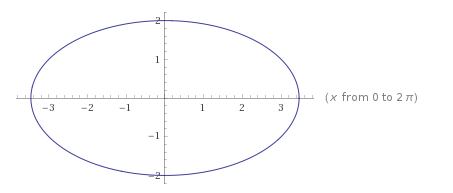
\includegraphics[width=14cm]{rozrahunkova_02/04_02.png}
  \caption{Параметрично заданий еліпс}
  \label{fig:rr_01_40_02}
  \centering
\end{figure}

Оскільки фігура площу якої ми шукаємо симетрична, ми будемо шукати її площу лише на відрізку її четверті (на відризку з $\pi/2$ до 0), а потім отриману площу просто помножим на 4.

$$
  \int^0_{\frac{\pi}{2}} 2 \sin{\varphi} (2\sqrt{3}\cos\varphi)' \d{\varphi}
= 2 \int^0_{\frac{\pi}{2}} \sin{\varphi} \times (- 2\sqrt{3} ) \sin{\varphi} \d{\varphi}
= -4\sqrt{3} \int^0_{\frac{\pi}{2}} \sin^2{\varphi} \d{\varphi}
$$
$$
  -4\sqrt{3} ( \dfrac{\varphi}{2} - \dfrac{\sin{2\varphi}}{4} ) \Bigg|^0_{\frac{\pi}{2}}
= -\dfrac{4\sqrt{3}}{2} ( \varphi - \dfrac{\sin{2\varphi}}{2} ) \Bigg|^0_{\frac{\pi}{2}}
= -2\sqrt{3} ( 0 - \dfrac{\sin{2 \times 0}}{2} - ( \dfrac{\pi}{2} - \dfrac{\sin{2 \times \dfrac{\pi}{2} }}{2} ) )
$$

$$
= -2\sqrt{3} ( 0 - \dfrac{\sin{0}}{2} -   \dfrac{\pi}{2} + \dfrac{\sin{\pi}}{2} )
= -2\sqrt{3} ( 0 - 0 - \dfrac{\pi}{2} + 0 )  =  -2\sqrt{3} \times -\dfrac{\pi}{2}
= \boxed{\pi\sqrt{3}}
$$

Оскільки ми шукали площу лише четверті еліпсу, домножимо отриману площу на 4 щоб знайти повну площу.

$$
  \boxed{S = 4\pi\sqrt{3}}
$$

%
% http://mathprofi.ru/ploshad_i_obyem_esli_linija_zadana_parametricheski.html
%
